%%%%%%%%%%%%%%%%%%%%%%%%%%%%%%%%%%%%%%%%%%%%%%%%%%%%%%%%%%%%%%%%%%%%%%%%%%%%%%%%
%
%   .x~~"*Weu.
%  d8Nu.  9888c
%  88888  98888
%  "***"  9888%
%       ..@8*"
%    ````"8Weu
%   ..    ?8888L
% :@88N   '8888N
% *8888~  '8888F
% '*8"`   9888%
%   `~===*%"`
%
%%%%%%%%%%%%%%%%%%%%%%%%%%%%%%%%%%%%%%%%%%%%%%%%%%%%%%%%%%%%%%%%%%%%%%%%%%%%%%%%

\documentclass[../paper.tex]{subfiles}
\begin{document}

\chapter{Co-Design}
\label{codesign}

In section~\ref{embedded} we introduced a simplified version of our co-design, vector and signal languages to illustrate embedded programming in Haskell. We then went on to implement two versions of an FIR filter, one with vectors and one with signals. For the kind of heterogeneous computing our co-design language aims to describe, the simplified types we have shown so far are not enough. Heterogeneous systems typically see hardware code interleaved with software code, and our language therefore needs to be able to describe both. To facilitate design exploration we also need to support descriptions that are not restricted to either language, but rather the operations they require.

C and its dialects are perhaps the most commonly used languages for writing software in embedded systems. The co-design language is no different and compiles its software programs to C as well. For hardware descriptions, we use the VHDL language. This decision is purely based on the fact it is the hardware description language we are most comfortable with. Neither choice of language is final, and the language does support the addition of new target languages. Furthermore, both software and hardware are extensible and can be adapted to describe a multitude of embedded systems.

Starting with a single Haskell program, our co-design library is designed with three main tasks in mind: generate C code for the software parts, VHDL for the hardware parts, and to generate a combination of software and hardware for the transmission of data between components.

\section{Hardware Software Programs}
\label{program}

C and VHDL are different from one another in that one describes software code and the other hardware designs, although both languages use an imperative style of programming. The co-design language is therefore built on a deep embedding of monads as a representation of imperative programs---remember that monads can be thought of as composable descriptions of computations, that is, they provide a means to connect smaller programs into a single, larger program.

The general idea behind a monadic embedding is that one can view an imperative program as a sequence of instructions to be executed on some machine---which looks similar to programs written in a stateful monad using Haskell's do-syntax. In fact, a stateful program composed with monadic operations can be directly translated into statements in an imperative language. As an example of these similarities, consider a software program for reversing an array:

\begin{code}
reverseS :: SArr Int32 -> Software ()
reverseS arr =
  for 0 (len `div` 2) $ \ix -> do
    aix <- getArr arr ix
    ajx <- getArr arr (len - ix - 1)
    setArr arr ix ajx
    setArr arr (len - ix - 1) aix
  where
    len = length arr
\end{code}

The implementation of \codei{reverseS} certainly has the look and feel of a imperative program, sans a few syntactical differences. Its type signature tells us that it takes an array over signed integers as input and produces a software program---notice that the array type \codei{SArr} is prefixed with an \codei{S} in order to show that it is intended to be used with software statements. The return type is empty since the array is reversed in place.

While the type of \codei{reverseS} is that of a software program, there's nothing software specific about its implementation. For-loops and arrays are both part of most imperative languages, including C and VHDL. We could just as well have implemented reverse as a hardware function. In fact, we can define the hardware version by simply changing the previous function's type signature while keeping its body intact:

\begin{code}
reverseH :: HArr Int32 -> Hardware ()
reverseH arr =
  for 0 (len `div` 2) $ \ix -> do
    aix <- getArr arr ix
    ajx <- getArr arr (len - ix - 1)
    setArr arr ix ajx
    setArr arr (len - ix - 1) aix
  where
    len = length arr
\end{code}

The similarity between \codei{reverseS} and \codei{reverseH} hint that a software or hardware type for reverse is unnecessarily restrictive. A function type that is not limited to either language, but rather the functionality it requires, can be expressed in the co-design language thanks to type classes it provides. These classes are used to ensure a type provides the functionality a program requires, like \codei{Num} did for the numerical expressions in section~\ref{embedded}. That is, we can replace the software and hardware types with a generic program type and then add constraints for any functionality we require.

Going back to our reverse example, we can give it the following generic type:

\begin{code}
reverse :: (Monad m, Arrays m, Control m, TypeM m Int32)
        => Arr m Int32 -> m ()
\end{code}

\noindent \codei{SArr} and \codei{HArr} are substituted for the generic array type \codei{Arr}, which is parameterized on the monad \codei{m}. Such an associated type for arrays lets us talk about the array type of \codei{m}; \codei{Arr} will turn into either \codei{SArr} or \codei{HArr} when \codei{m} is instantiated as the software or hardware monad.

Three new constraints were introduced for the generic reverse, namely \codei{Arrays}, \codei{Control}, and \codei{TypeM}. The first two ensure that \codei{m} supports arrays and for-loops, whereas the third one states that signed integers is a valid type in \codei{m}. \codei{Arrays} and \codei{Control} are defined as follows:

\begin{code}
class Monad m => Arrays m where
  type Arr m
  newArr :: TypeM m a => Exp m Length -> m (Arr m a)
  getArr :: TypeM m a => Arr m a -> Exp m Index -> m a
  setArr :: TypeM m a => Arr m a -> Exp m Index -> a -> m ()

class Monad m => Control m where
  for :: (TypeM m a, Integral a) => Exp m a -> Exp m a -> (Exp m a -> m ())
      -> m ()
\end{code}

\noindent Each class lists the functions it provides and in the case of arrays, the type to use with them; \codei{Exp} represents the expression type associated with \codei{m}. Seeing as these operations are quite common, we give a short-hand for a collection of them plus references:

\begin{code}
type MonadComp m = (Monad m, References m, Arrays m, Control m)
\end{code}

Just as there are classes of operations, that both software and hardware support, there are also operations that some languages support but others do not. The type classes therefore form a hierarchy. Monads form the base of the class hierarchy, but functions intended for either software or hardware branches also require that \codei{m} is an extension of their respective monads. For example, processes in hardware are given by the following type class:

\begin{code}
class HardwareMonad m => Process m where
  process :: m () -> m ()
\end{code}

At this point we should note that types introduced in this section are slightly different from those found in section~\ref{embedded}. For instance, the array type now has an extra parameter \codei{m}. The earlier types are in fact synonyms for the software types introduced in this section, and served to give a simplified introduction to the co-design language. We reimplement the dot-product using the new types as a comparison to the old:

\begin{code}
dot :: (MonadComp m, TypeM m a, Num a) => Arr m a -> Arr m a -> m (Exp m a)
dot x y = do
  sum <- initRef 0
  for 0 (min (length x) (length y) $ \ix -> do
    a <- getArr x ix
    b <- getArr y ix
    modifyRef sum $ \s -> s + a * b
  getRef sum
\end{code}

\noindent The function's type has changed, as expected, but its body remains the same as before.

The programs we have show in this section are simply a convenient model of imperative programs and, from a users perspective, can be rather clunky. Nevertheless, they are easy to compile down to source code, and the next section goes into their representation and interpretation in detail. Later chapters show how programs is also a convenient translation target for vector computations and signal processing networks.

% As an example of a larger function, we also implement the full FIR filter. The filter itself is fairly straightforward: inputs are shifted onto the taps one by one and for each input the current impulse response is calculated using a dot-product:

%\begin{code}
%fir :: (MonadComp m, TypeM m a, Num a) => Arr m a -> Arr m a -> m (Arr m a)
%fir bs xs = do
%  taps <- newArr (length bs)
%  ys   <- newArr (length xs)
%  for 0 (length bs) $ \ix -> setArr taps ix 0
%  for 0 (length xs) $ \ix -> do
%    for 1 (length bs) $ \jx -> do
%      tmp <- getArr taps (jx - 1)
%      setArr taps jx tmp
%    x <- getArr xs ix
%    setArr taps 0 x
%    o <- dot bs taps
%    setArr ys ix o
%  return ys
%\end{code}

% While the above implementation is suitable for a software, it is perhaps not ideal as a hardware design. Signal processing in C is often done with arrays over chunks of the input, while a hardware is build around signals and processes to drive a continuous filter. Assuming a hardware description is our goal, the necessary change is however quite small: we swap the input and output arrays for signals and change the outer for-loop into a process. Rewriting programs at this scale is a kind of optimization we think developers are comfortable with.

\section{Instructions}
\label{instr}

The co-design language is inspired by the work of Josef and Joel~\cite{BjornBenny} and by the Operational Monad~\cite{Operational} and is as such based on a monadic representation of imperative programs. Like our inspiration, the program type is deeply embedded in order to capture a computation as an algebraic data type and parameterized on the instructions used in said computations. Unlike previous work, we also take into account the fact that different languages will support different expressions, types, etc. Some might even share a sub-set of each others instructions but include a few of their own primitives---we would rather not copy an entire language just to add a new primitive. We have thus taken extra care to make sure instructions, and to some extent the expressions, can be defined compositionally. The program type is therefore parameterized on its instructions, as before, but also includes a type-level list for the other types associated with the language:

\begin{code}
data Program instr fs a
\end{code}

The general idea behind the program type is that it allows for instructions to be separated from their sequencing, since an instruction's effect will only depend on its interaction with other instructions. That is, Haskell's monadic syntax ensures that any instructions we use in our programs are sequenced correctly. As a consequence of this separation, the task of implementing a language based on programs is the same as writing an interpreter for the language's instructions. In particular, we can define a generic interpreter for programs that maps them to their intended meaning:

\begin{code}
interpret :: (Interp i m fs, HFunctor i, Monad m) => Program i fs a -> m a
\end{code}

\codei{interpret} lifts a monadic interpretation of instructions, which may be of varying types, to a monadic interpretation of the whole program. By using different types for the monad \codei{m}, it is possible to implement different ``back ends'' for programs. For example, interpretation in Haskell's \codei{IO} monad gives a way to \emph{run programs}, while interpretation in a code generation monad can be used to make a \emph{compiler}. The interpretation of an instruction set \codei{instr} to the monad \codei{m} is given by \codei{Interp}:

\begin{code}
class Interp instr m fs where
  interp :: instr (P2 m fs) a -> m a
\end{code}

\noindent where \codei{P2} is a synonym for a parameter list of two elements, here \codei{m} and \codei{fs}. Note also that \codei{interpret} also require that its instructions are higher-order functors:

\begin{code}
class HFunctor h where
  hfmap :: (forall b . f b -> g b) -> h (P2 f fs) a -> h (P2 g fs) a
\end{code}

Higher-order instructions, parameterized on the program they are part of, makes it possible to define instruction sets compositionally using, for instance, a technique like Data Types \`{a} La Carte~\cite{DTC}. Extensible instructions sets are particularly useful for our co-design language, as any existing hardware and software instructions can be reused for new systems; we only need to add support for new intrinsic instructions and expressions. That is, to extend either the hardware or software language, we only need to add a data type of our new primitive, define a new set of instructions that includes it, and add support for its interpretation. 

% In the original Operational Monad this could be only done for simple instructions, but with our new program type it can be done even for \emph{control instructions}---instructions that take programs as arguments.

As an example of how a new instruction can be defined, we introduce the \codei{If} construct:

\begin{code}
data ControlCMD fs a where
  If :: exp Bool -> prog () -> prog () -> ControlCMD (P3 prog exp pred) ()
\end{code}

\noindent The type parameter \codei{prog} refers to sub-programs, \codei{exp} refers to pure expressions, and \codei{pred} refers to type predicates. Although \codei{pred} is not used in the definition of \codei{If}, it is used by other instructions and therefore included here to keep the parameter lists consistent. \codei{P3} is a synonym for a parameter list of three arguments.

Assuming we have access to a few other instructions like \codei{If}, we can now define a program type that combines several instructions in a Data Types \`{a} La Carte fashion:

\begin{code}
type MyProgram exp pred = Program (If :+: Reference :+: ...) (P2 exp pred)
\end{code}

\noindent The recursive program type will then set the type of sub-programs in \codei{If} to \codei{MyProgram}.

The final step to our extension is to add support for interpreting \codei{MyProgram}, that is, we must define an instances for \codei{Interp} and \codei{HFunctor}. Fortunately, both classes distribute over \codei{(:+:)}, so we need only define instances for \codei{If}. The \codei{HFunctor} instance is defined as:

\begin{code}
instance HFunctor ControlCMD where
  hfmap f (If c thn els) = If c (f thn) (f els)
\end{code}

\noindent While interpretation in, for example, the \codei{IO} monad could look as follows:

\begin{code}
instance Interp ControlCMD IO fs where
  interp (If b tru fls) = if evalExp b then tru else fls
\end{code}

\noindent where \codei{evalExp} is an evaluator for the expression language.

\section{Expressions}
\label{expr}

A language embedding based on monads gives us a representation of the statements in an imperative program, but most meaningful programs also include a notion of pure expressions. These expressions contain a combination of one or more values, constants, variables and operators that our co-design library interprets and computes to produce a value. As a small example, consider a function for squaring a value:

\begin{code}
square :: (Num (exp a), Type exp a) => exp a -> exp a
square a = a * a
\end{code}

\noindent Note that the \codei{Type} constraint on \codei{a} is slightly different than \codei{TypeM} from section~\ref{program}, as \codei{Type} accepts expressions rather than monads for its first argument.

% that before as we use \codei{Type} instead of \codei{TypeM}: the former is designed to be used with expressions rather than monads.

Programming with expressions in our co-design language is evidently quite similar to how its done in regular Haskell. For instance, applying the squaring function to a value of $5$ is equivalent to the mathematical expression $5*5$ which evaluates to $25$. The expressions used in our co-design language are however deeply embedded, and as we saw in section~\ref{domain}, that means evaluation isn't the only interpretation they can support. In fact, by substituting the general \codei{exp} type for either the software or hardware expression type, \codei{SExp} and \codei{HExp}, expressions can be compiled as well.

In simple expressions, like the above squaring function, the resulting value is usually one of the various primitive types, such as signed and unsigned numerical, floating point, or logical. In more elaborate expressions it can however be a complex data type. We can, for example, define an expression that consists of a pair of values:

\begin{code}
dist :: (SExp Float, SExp Float) -> (SExp Float, SExp Float) -> SExp Float
dist (x1, y1) (x2, y2) = sqrt (dx**2 + dy**2)
  where
    dx = x1 - x2
    dy = y1 - y2
\end{code}

\noindent \codei{dist} computes the distance between two points in a plane, where points are represented as a pair of coordinates. The pairs are simply syntactic suger, and will not appear in the generated code.

In addition to the numerical and logical functions we have seen so far, expressions also provide a number of abstractions that we are accustomed to as functional programmers:

\begin{code}
class Let exp where
  share :: (Type exp a, Type exp b) => exp a -> (exp a -> exp b) -> exp b
\end{code}

Abstractions like the let-binding are one of the hallmarks of functional programming and let users avoid unnecessary detail and mundane operations. At the same time, such abstractions can complicate the compiler and make it harder to generate efficient code. To circumvent this problem, the co-design language makes use of two expression types: one with only primitive operations that is easy to compile, and one with features like let-bindings that is comfortable to program with. Seeing as the feature rich expression type is an extension of the basic one, the two does inevitable share a few primitives and are therefore defined using a technique similar to Data Types \`{a} La Carte---like the instructions from section~\ref{instr}.

In order to avoid having separate instances of each interpretation for the two expression types, which is a tedious and error-prone task, we provide an elaboration from the feature rich expressions into program snippets over the primitive expressions:

\begin{code}
elaborateSExp :: SExp a -> Program SIns (P2 CExp SType) (CExp a)
\end{code}

\noindent Here, \codei{SIns} and \codei{SType} are the software instruction set and type predicate, and \codei{CExp} is the primitive software expressions. The program wrapping is necessary in order to translate some expressions as, for instance, let-bindings use references to hold its shared value.

\codei{elaborateSExp} provides a means to elaborate a single expression. For a full program, we need to elaborate every expression an instruction contains. Programs are fortunately monads, and its thus possible to use the earlier \codei{interpret} function from section~\ref{instr} to elaborate entire programs---assuming we use \codei{elaborateSExp} to give an instance of \codei{Interp} for expressions. For example, a whole software program can be elaborated as:

\begin{code}
elaborateSoft :: Software a -> Program SIns (P2 CExp SType) a
elaborateSoft = interpret
\end{code}

An evaluator for software programs can then defined by combining the elaboration of expressions with an interpreter for the simpler software expressions and instructions:

\begin{code}
runSoft :: Software a -> IO a
runSoft = interpert . elaborateSoft
\end{code}

This interpretation of expressions have a few benefits: it is typed, which rule out many potential errors; it is easier to write than a complete translation into source code; the low-level expression type is reusable and can be used as an elaboration target for multiple, higher-level expression types.

\section{Components}

The ability to write a program that is constrained to its required functionality, rather than a specific language, means that users can easily experiment with putting their functions on different components in a system. Most interesting heterogeneous programs do however include a mixture of software and hardware fragments where the different parts communicate with each other. In the kind of FPGAs with embedded systems that we consider, communication is typically done over an AXI4 or AXI4-lite interconnect. 

Full AXI4 offers a range of interconnects that include variable data and address bus widths, high bandwidth burst and cached transfers, and various other transaction features that makes it useful for streaming. A lighter version of the AXI4 interconnect is offered through AXI4-lite, which is a subset of the full specification that forgoes the streaming features for a simpler communication model that writes and reads data one piece at a time. While full AXI4 certainly has its uses, we have opted to implement the AXI4-lite interconnect---the lighter interconnect offered by AXI4-lite is a better fit for our examples.

Five channels make up the bulk of the AXI4-lite specification: the read and write address channels, the read and write data channels, and the write acknowledge channel. These five channels are represented in VHDL as signals, driven by processes that implement the associated handshaking and logic for reading and writing. Signals behave very much like the references found in C, and a process is a kind of function that runs automatically once any of its inputs change. Both signals and processes are supported by our co-design language and a whole AXI4-lite interconnect is in fact implemented within the language as a function called \codei{axi4lite}. The function takes a hardware component and connects it to the read and write channels of a new interconnect:

\begin{code}
axi4lite ::
     Component a
  -> Component (
          Sig (Bits 32) -- Write address.
       -> Sig (Bits 3)  -- Write channel protection type.
       -> Sig Bit       -- Write address valid.
       -> Sig Bit       -- Write address ready.
       -> Sig (Bits 32) -- Write data.
       -> Sig (Bits 4)  -- Write strobes.
       -> Sig Bit       -- Write valid.
       -> Sig Bit       -- Write ready.
       -> Sig (Bits 2)  -- Write response.
       -> Sig Bit       -- Write response valid.
       -> Sig Bit       -- Response ready.
       -> Sig (Bits 32) -- Read address.
       -> Sig (Bits 3)  -- Protection type.
       -> Sig Bit       -- Read address valid.
       -> Sig Bit       -- Read address ready.
       -> Sig (Bits 32) -- Read data.
       -> Sig (Bits 2)  -- Read response.
       -> Sig Bit       -- Read valid.
       -> Sig Bit       -- Read ready.    
       -> ())
\end{code}

\noindent Or if we're only interested in a design of the interconnect:

\begin{code}
compileAXILite :: Component a -> String
\end{code}

\noindent Signal names in the generated interconnect all follow the AXI4-lite standard, and should as such be automatically recognized by most synthesizers as a AXI4 component. We show how to synthesize the design manually with the 2015.2 version of Vivado~\cite{feist2012}---the hardware project we're using for our target system requires this specific version. The actual design we're putting onto the FPGA is not important at this point, as the steps outlined below are the same for all designs. 

Firstly, we create a project for the AXI4 component, and we will use Vivado's tools to give us a template to start from. In particular, we use the ``Create and Package IP'' option under ``Tools'' to launch the creation wizard for a new AXI4 peripheral. Witch we then use to create a AXI4-lite slave, add it to our catalog of IP, and open a editing session for it. Two design files should now exist in our Vivado editor, as show in Figure~\ref{fig:files}.

\begin{figure}[t]
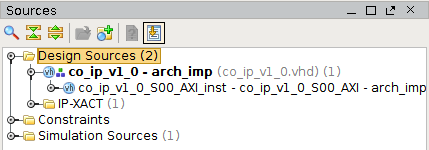
\includegraphics[width=0.4\textwidth]{figures/DesignFiles}
\centering
\caption{Design files generated for a AXI4 peripheral.}
\label{fig:files}
\end{figure}

The first file, which is called \codei{co_ip_v1_0} in our example, contains a shell for calling an AXI4-lite slave, and any other we might want to add to the same address space. The second file, called \codei{co_ip_v1_0_S00_AXI_inst}, contains an empty AXI4-lite slave. Its this second file that we substitute with our own design. Note that, after updating the second design, we need to make sure any references from the other design is updated as well. Once that’s done the project can be reviewed and packaged---the review will probably complain that an address port has changed in size, as we always use the full 32 bits rather than a subset, so go ahead and update its size accordingly.

With our AXI4-lite peripheral saved and packaged, we open up the main project. The system we target is one based on the Zynq board and contains two embedded ARM cores, an FPGA, and possibly a few other accelerators and co-processors, we are however only interested in the first two for now. The block design of our system is given by Figure~\ref{fig:zynq}.

\begin{figure}[h]
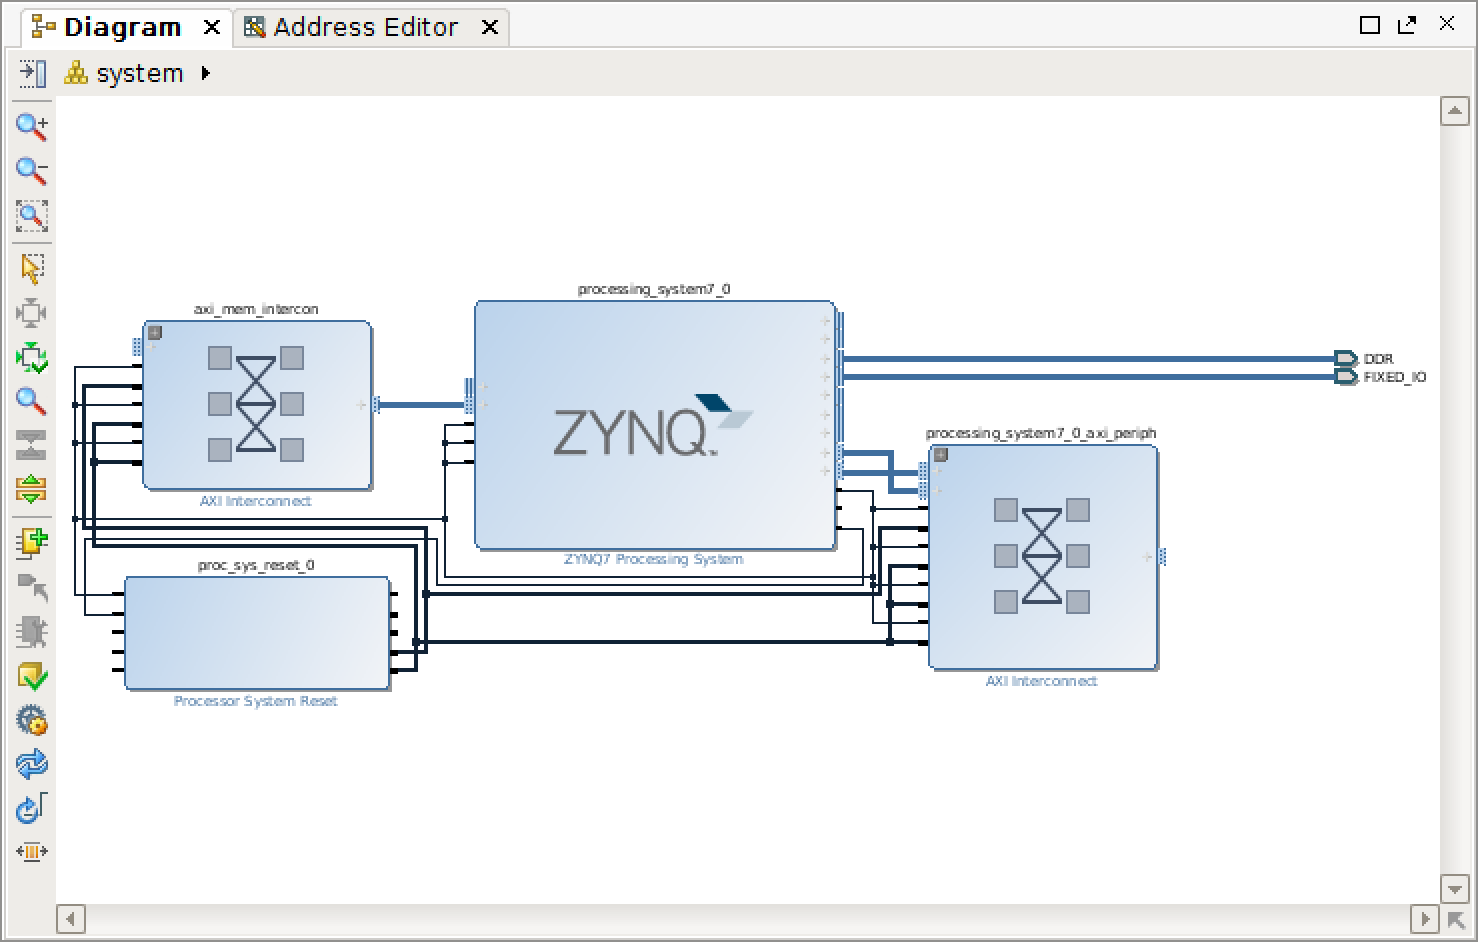
\includegraphics[width=0.4\textwidth]{figures/Zynq}
\centering
\caption{Base Zynq project.}
\label{fig:zynq}
\end{figure}

Loading our AXI4-lite peripheral into the main project is straightforward: under the ``IP Settings'' menu, we have the option to locate our newly created project and add it as a repository, from which we can then add its AXI4-lite slave component as an ``IP'' to our main project. With the component added, Vivado can hook it up to our main system automatically through its ``Run Connection Automation'' tool. Finally, we generate a bitstream to put onto the FPGA and get its physical address from the ``Address Editor''. The block design final block design is given by Figure~\ref{fig:system}, and its implementation is given by Figure~\ref{fig:design}.

\begin{figure}[h]
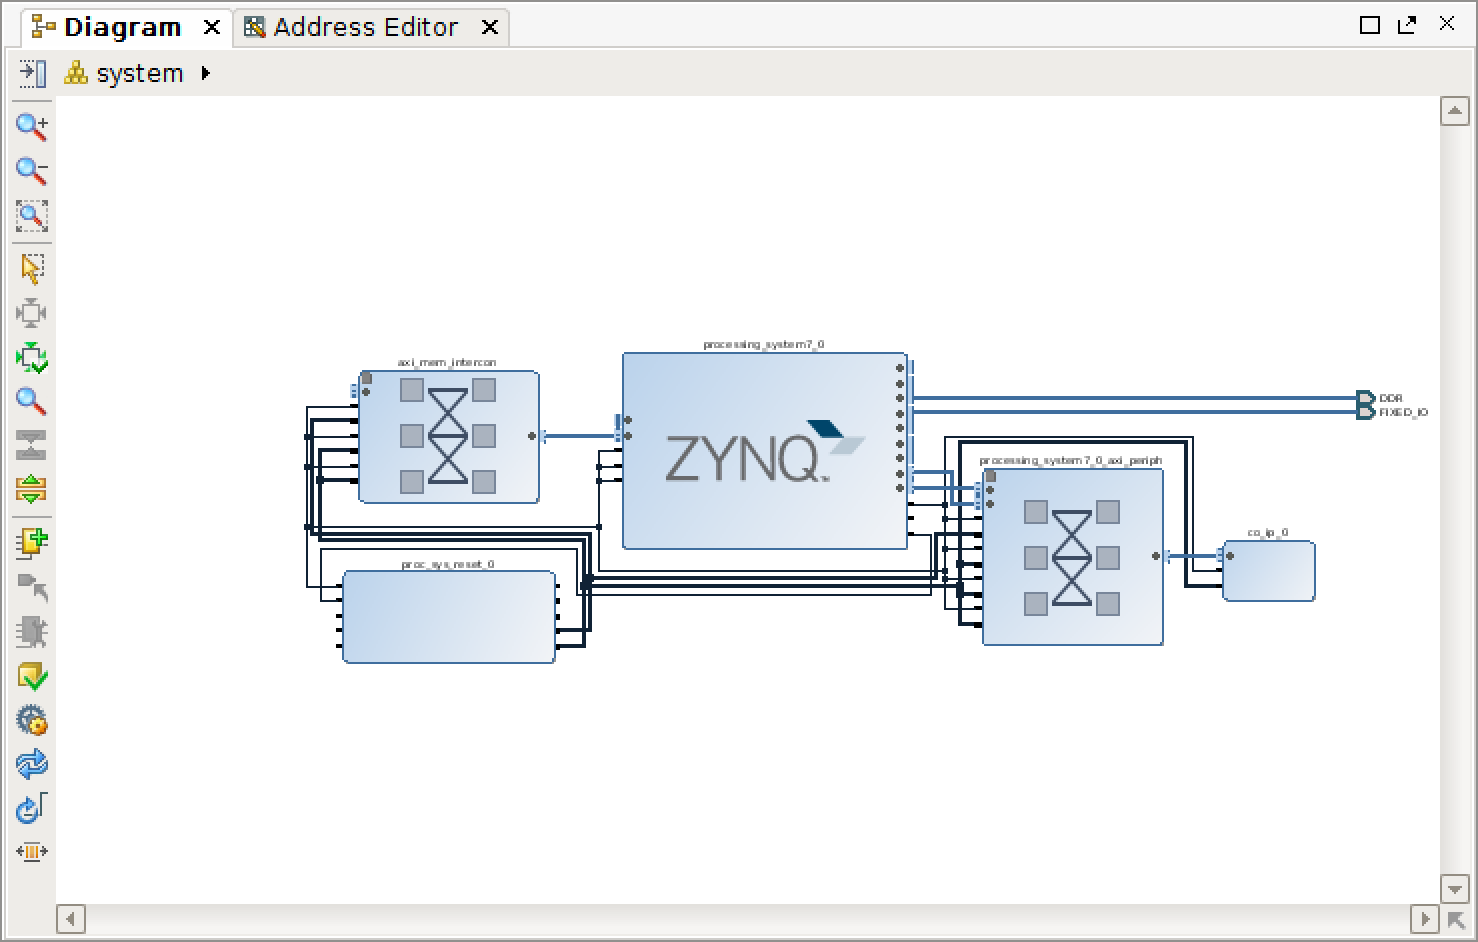
\includegraphics[width=0.4\textwidth]{figures/ZynqSystem}
\centering
\caption{Zynq project with AXI4-lite peripheral.}
\label{fig:system}
\end{figure}

\begin{figure}[h]
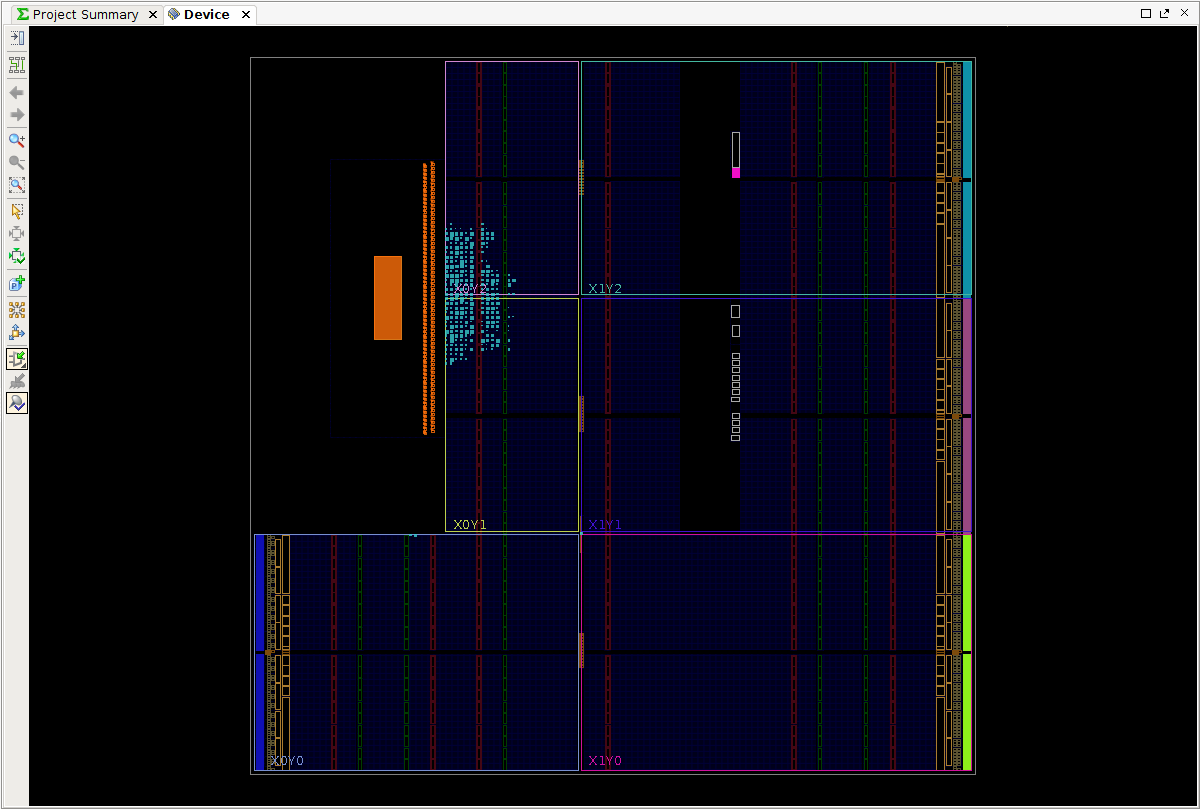
\includegraphics[width=0.4\textwidth]{figures/ZynqDesign}
\centering
\caption{Implementation of the project.}
\label{fig:design}
\end{figure}

Hardware components on the FPGA can interface with each other using port-maps as usual, but with the physical address of a component, it is also possible to access it from software with memory-mapped I/O. The general idea is that memory-mapping a component causes it to share its address space with the memory of whatever software program is running, that is, a component can be reached from software by simply writing to and reading from pointers to its address. The software function \codei{mmap} preforms the necessary memory-mapping for a component:

\begin{code}
mmap :: Address -> Component a -> Software (Pointer (Soften a))
\end{code}

\noindent Note that the resulting memory pointer of \codei{mmap} has ``soften'' its component's original type. Softening refers to the process of replacing any hardware specific types, like signals, with their corresponding type in software, and is described by the type family \codei{Soften}:

\begin{code}
type family Soften a where
  Soften (Sig a -> b) = SRef a -> Soften b
  --dotLine
\end{code}

A softened pointer can then be called from software with a matching set of arguments:

\begin{code}
call :: Pointer a -> Argument a -> Software ()
\end{code}

\noindent As \codei{call} goes through the argument list writes each value marked as input to the memory pointer---different input signals are reached by simply offsetting the address---and output values are read in a similar manner. The component's output can then be read from the argument matching its output signal. As for the argument list, it is a typed heterogeneous list that ensures we use the expected number of arguments and that all intermediate types match. A list of arguments is constructed with the following functions:

\begin{code}
nil   :: Argument ()
(:>)  :: SType a => SRef a -> Argument b -> Argument (SRef a -> b)
(:>>) :: SType a => SArr a -> Argument b -> Argument (SArr a -> b)
\end{code}

\noindent \codei{nil} creates an empty argument list, and the two infix functions \codei{(:>)} and \codei{(:>>)} extends an argument list with a reference and an array, respectively.

As an example of offloading a function to hardware, we revisit the earlier dot product from section~\ref{program} and recall that it had the following type:

\begin{code}
dot :: (MonadComp m, TypeM m a, Num a) => Arr m a -> Arr m a
  -> Program (Exp m a)
\end{code}

\noindent While we as designers can read the dot-products type, other functions cannot. So, before we can hook up the dot-product to an AXI4-lite interconnect and offload it, we need to give it a type signature that can be read by other functions. Seeing as the dot-product takes two arrays as input and then produces an expression as output, we can give it the following signature:

\begin{code}
comp :: Component (HArr Int32 -> HArr Int32 -> Signal Int32 -> ())
comp = inputArr 3 $ \a -> inputArr 3 $ \b -> returnC $ dot a b
\end{code}

\noindent Where \codei{inputArr} adds an array of a given length to the signature, and \codei{returnC} rounds of the type signature with a signal for the dot product's output. The wrapped \codei{dot} can be hooked up to an interconnect with \codei{axi4lite} and then be compiled, synthesized and put onto hardware.

In order to communicate with our offloaded dot-product from software we need to get its physical address from the synthesis tool, which is ``0x4C300000'' in our case. With the address in hand we can now put together a small software program that call our dot-product and print its result to standard output:

\begin{code}
program :: Software ()
program = do
  dot <- mmap "0x4C300000" comp
  arr <- initArr [1 .. 3]
  brr <- initArr [3 .. 6]
  res <- newRef
  call dot (arr :>> brr :>> res :> nil)
  val <- getRef res
  printf "%d\n" val
\end{code}

\section{Vectors}
\label{vectors}

Sequential programs in the co-design language makes use of its array type to express array and vector computations with mutable updates. These arrays provide full control over their allocation and assignment, but do so through a low-level and imperative interface. As we saw in section~\ref{embedded}, some functions are better expressed in a compositional manner than as a sequential program. To facilitate the design of array and vector functions, we provide the vector language. 

A typical vector computation starts with a ``manifest'' vector, that is, a vector which refers directly to an array in memory. Vector operations are then applied, where each operation is overloaded to accept any ``pully'' vector as input and produces another ``pully'' vector. Then, once the various vectors have been constructed, they are assembled into a ``pushy'' vector and written to memory, resulting in a new ``manifest'' vector. The various names for ``manifest'', ``pully'' and ``pushy'' vectors draw inspiration from the Pan language~\cite{elliott2003} and push arrays~\cite{claessen2012}, the ideas of which our vectors are based on.

Manifest vectors are more often than not the immutable arrays provided by the co-design language, as such arrays have an representation in memory. A Push vector on the other hand is not stored in memory, but is rather represented as a function:

\begin{code}
data Pull exp a where
  Pull :: exp Length -> (exp Index -> a) -> Pull exp a
\end{code}

\noindent A pull vector consists of a length---the number of elements in the vector---and a function that given an index in the vector returns an element. Furthermore, pull vectors are designed in such a way that all operations fuse together without creating any intermediate structures in memory, a property which is often referred to as vector fusion.

Push vectors go in the opposite direction of pull vectors, and give us control over a vectors evaluation to the producers rather than the consumer. That is, pull vectors have a representation that supports nested writes to memory and fusion of operations. Push vectors are represented as:

\begin{code}
data Push m a where
  Push :: Exp m Length -> ((Exp m Index -> a -> m ()) -> m ()) -> Push m a
\end{code}

\noindent A push vector consists of a length, like pull vectors, but their function describes how elements are evaluated rather then how they are fetched. As such, they are parameterized on the type \codei{m} rather than an expression type; \codei{Exp} is an associated type, like \codei{Arr} from section~\ref{codesign}, and refers to the expression type associated with \codei{m}. The general idea is to instantiate \codei{m} as either of the co-design's two languages and have the push vector's function write each element to an array. In particular, push arrays implement efficient concatenation and interleaving, which would otherwise introduce unnecessary conditionals had they been implemented with pull vectors.

As an example, consider the sum of the square of all numbers from zero to $n$:

\begin{code}
squares :: (Num a, Type exp a) => exp a -> exp a
squares n = sum $ map (\x -> x * x) (1 ... n)
\end{code} %$

\noindent Note that no vector occurs in the function's type, but they are used internally to compute the result: the infix function \codei{(...)} constructs a pully vector with values from one to $n$, to which a mapping is applied that squares each element. The vector is then converted into a push vector and summed up into a single value.

Each vector type has a different set of operations associated with it, and these operations are chosen in such a way that each vector type only supports those operations which can be performed efficiently for that type. In many cases, the vector type is guided by the types of the operations involved, and follows the typical pattern of a manifest vector being turned into a pull vector, which turns into a push vector, which is then written to memory and turns back into a manifest vector. There are however cases where its preferable to ``skip'' parts of the cycle. For instance, the \codei{squares} function starts with a pull vector rather than a manifest vector.

The functions associated with each kind of vector are overloaded in the kind of vectors they accept: an operation for a pull vector will support the use of any ``pully'' vector type. For instance, the \codei{sum} function used in the above \codei{squares} is defined as follows:

\begin{code}
sum :: (Pully exp vec a, Type exp a, Num a) => vec -> a
sum = fold (+) 0
\end{code}

\section{Signal processing}
\label{signals}

While the imperative style of programming of the co-design language is already convenient for software realization, section~\ref{embedded} did show that a compositional description can give us a better intuition of what a program consists of. Section~\ref{vectors} addressed this deficiency as its vectors provide a comfortable syntax for composing smaller array functions to form a larger program. For functions that involve a notion of time, we have signals.

The signal language is based on the concept of signals: possibly infinite sequences of values in some pure expression language, given by the type \codei{Sig}. Conceptually, signals can be thought of as infinite lists. Unlike lists however, a signal is not a first-class value and cannot be nested---we cannot construct a signal over other signals. Programming with signals is done compositionally, that is, a signal program is a collection of mutually recursive signal functions, each built from repeating values or other signals:

\begin{code}
repeat :: pred a => exp a -> Sig exp pred a

map :: (pred a, pred b)
  => (exp a -> exp b)
  -> Sig exp pred a -> Sig exp pred b

zipWith :: (pred a, pred b, pred c)
  => (exp a -> exp b -> exp c)
  -> Sig exp pred a -> Sig exp pred b -> Sig exp pred c
\end{code}

These signal functions model the similarly named functions in Haskell base libraries: \codei{repeat} creates a signal by repeating some value, \codei{map} applies a function to each value of a signal, and \codei{zipWith} joins two signals element-wise using then given function. The idea is to mimic the kind of compositional programming that users normally do in Haskell, or using vectors. Ground types in the expression language are lifted to operate element-wise over signals as well, typically with a type class like \codei{Num}:

\begin{code}
instance (Num (exp a), pred a) => Num (Sig exp pred a) where
  fromInteger = repeat . fromInteger
  (+)         = zipWith (+)
  (-)         = zipWith (-)
  --dotLine
\end{code}

All signal functions we have shown so far have been combinatorial, in the sense that their output only depends on the current inputs. Sequential functions on the other hand needs to access older values. For these, the signal language provides a unit delay:

\begin{code}
delay :: pred a => exp a -> Sig exp pred a -> Sig exp pred a
\end{code}

\noindent \codei{delay} prepends a value to a signal, delaying its original output by one time instant---the function introduces the notion of a \emph{next time step}, making time enumerable. While \codei{delay} may appear innocent, combined with feedback it can describe any kind of sequential signal network. For example, a parity checker can be defined as:

\begin{code}
parity :: Sig exp pred Bool -> Sig exp pred Bool
parity inp = out where
  out = zipWith xor (delay false out) input
\end{code}

As a larger example, we implement a infinite impulse response (IIR) filter, which comprises the second primary type of digital filters used in digital signal processing applications and, unlike FIR filter in section~\ref{embedded}, contains feedback. The IIR filter is typically described and implemented in terms of a difference equation:

\begin{equation}
y_{n} = {1 \over a_{0}} \: \cdot \: \left( \sum_{i=0}^{P} b_{i} \cdot x_{n-i} \: - \: \sum_{j=1}^{Q} a_{j} \cdot y_{n-j} \right)
\end{equation}
\vspace{1mm}

\noindent $P$ and $Q$ are the feed-forward and feedback filter orders and $a_{j}$ and $b_{i}$ are the filter coefficients. Note that $a_{0}$ is used in the outer division and is not part of the feedback sum.

Examining the above equation we can see that the IIR filter loosely consists of two FIR filters, where the second filter has an extra delay and is recursively defined on its output. As such, we can reuse the FIR filter from section~\ref{embed} and define the filter as:

\begin{code}
iir :: (Fractional a, Num (exp a), pred a) => exp a -> [exp a] -> [exp a]
  -> Sig exp pred a -> Sig exp pred a
iir a0 as bs x = y
  where
    y = (1 / repeat a0) * (upper x - lower y)
    upper = fir bs
    lower = fir as . delay 0
\end{code}

A circular definition of \codei{y} in the IIR filter is possible thanks to the \codei{delay} operator, which ensures a productive network as each output only depends on previous input. In general we have that recursively defined signals introduce feedback, while recursion over Haskell values, like lists, can be used to build repeating graphs structures.

This behavior of \codei{delay} implies that we can distinguish values that have and haven't been delayed, which is something that's normally not possible to do in Haskell---being able to observe the sharing of \codei{y} will, by definition, break any referential transparency. In fact, the internals of \codei{delay} makes use of a restricted form of observable sharing~\cite{claessen1999, gill2009}. This allows us to turn signal functions like the above IIR filter into a directed graph. Any sharing is then visible as edges in the graph, connecting the nodes over its operations.

A graph representation of a signal network enables us to check for cycles, order its nodes, and compile it. Regular programs are however a poor target for signal functions, as its type loses any notion of streaming that a function might have had. So, a signal function is instead turned into a co-iterative stream~\cite{caspi1998}, where each stream has an initial state and a transition function from its current state to an output and a new state. The benefit of this approach is that it allows for infinite data types, like streams, to be handled in a strict and efficient way. The streams themselves are however based on programs:

\begin{code}
data Stream instr exp pred a where
  Stream :: Program instr (P2 exp pred) (Program instr (P2 exp pred) a)
    -> Stream instr exp pred a
\end{code}

\noindent A stream's outer program is used to initialize the stream, which results in another program that in turn produces the output values and updates the state.

\end{document}
